% !TEX program = xelatex
\documentclass[12pt,a4paper]{article}

% =================== PACKAGES ===================
\usepackage[T1]{fontenc}
\usepackage{geometry}
\usepackage{graphicx}
\usepackage{hyperref}
\usepackage{enumitem}
\usepackage{titlesec}
\usepackage{fancyhdr}
\usepackage{booktabs}
\usepackage{setspace}
\usepackage{newtxtext}        % Times-like serif (formal, academic)
\usepackage{parskip}          % Space between paragraphs
\usepackage[nottoc]{tocbibind}
\usepackage{tikz}
\usetikzlibrary{arrows.meta, positioning, shapes.geometric, backgrounds, calc}
\usepackage{caption}
\usepackage{float}
\graphicspath{{/Users/krust/Documents/eaClass/Seminar1/}}

% =================== PAGE LAYOUT ===================
\geometry{
  top=1in,
  bottom=1in,
  left=1.1in,
  right=1.1in,
  headheight=14pt
}
\setstretch{1.15}

% =================== HEADER / FOOTER ===================
\pagestyle{fancy}
\fancyhf{}
\fancyhead[L]{\small IK2015 \textemdash{} Enterprise Architecture and Database Programming}
\fancyhead[R]{\small Seminar 1: Project Proposal}
\fancyfoot[C]{\thepage}
\renewcommand{\headrulewidth}{0.4pt}

% =================== SECTION FORMATTING ===================
\titleformat{\section}[hang]{\Large\bfseries}{\thesection}{1em}{}
\titleformat{\subsection}[hang]{\large\bfseries}{\thesubsection}{1em}{}
\titlespacing*{\section}{0pt}{12pt}{6pt}
\titlespacing*{\subsection}{0pt}{10pt}{4pt}

% =================== HYPERLINK SETUP ===================
\hypersetup{
  colorlinks=true,
  linkcolor=black,
  citecolor=black,
  urlcolor=blue
}

% =================== TITLE AREA ===================
\title{}
\author{}
\date{}

\begin{document}

% ---- Custom Title Page ----
\thispagestyle{empty}
\vspace*{2cm}

\begin{center}
  {\normalsize Jiangxi University of Finance and Economics} \\[2.5cm]

  {\LARGE\bfseries Project Proposal} \\[1.2cm]

  {\Large Luckin Coffee Inc.} \\[0.3cm]
  {\normalsize\itshape A Technology-Driven New Retail Coffee Enterprise} \\[2.5cm]

  {\normalsize IK2015: Enterprise Architecture and Database Programming} \\[0.2cm]
  {\normalsize Seminar 1} \\[2.5cm]

  {\normalsize\textbf{Group 4}} \\[0.5cm]
  {\normalsize
    Zhe-Kai Yang~(Krust),\quad
    Shi-Hang Chen~(Sean),\quad
    Wei-Yu Cai~(Nosta), \\[0.2cm]
    Huan-Wen Chen~(Evan),\quad
    Yuan-Yong Liao~(Foreve)
  } \\[2cm]

  {\normalsize \today}
\end{center}

\newpage
\setcounter{page}{1}
\pagestyle{fancy}

% =================== I. TITLE ===================
\section{Project Title}
\noindent
\textbf{Luckin Coffee Inc.: A Technology-Driven Coffee Chain and New Retail Business Model.}

\vspace{0.3cm}

% =================== II. BUSINESS BACKGROUND ===================
\section{Background of the Selected Business}

\subsection{Corporate Overview}

Luckin Coffee Inc.\ (hereinafter ``Luckin'') was incorporated in 2017 and is headquartered in Xiamen, Fujian Province, People's Republic of China. Measured by store count, Luckin has ascended to become one of the largest coffee chains in China. Unlike incumbent competitors that have traditionally centred their business models on dine-in experiences and premium brand positioning, Luckin has pursued a fundamentally distinct strategic trajectory, constructing its operations around a technology-driven ``new retail'' paradigm. Under this model, the customer journey is predominantly mediated through digital interfaces---the Luckin mobile application or WeChat mini-program---through which consumers place orders, execute digital payments, select between in-store pickup and last-mile delivery, and monitor real-time order status. This architecture simultaneously reduces customer queuing time, elevates per-store throughput, and generates a continuous stream of transactional and behavioural data that feeds into product development, site-level operations, marketing automation, and supply chain orchestration.

\subsection{Products and Services}

Luckin's core offering encompasses freshly brewed beverages, with a particular emphasis on coffee- and tea-based drinks. Its product portfolio spans traditional espresso-based beverages (Americano, latte, cappuccino), specialty and flavoured coffee variants, fruit-infused coffee concoctions, light milk tea, and an array of ancillary food items including snacks and light meals. Beyond in-store consumption, Luckin has cultivated a complementary packaged-goods vertical, marketing instant coffee, whole-bean coffee, drip-bag coffee, capsules, and branded accessories through both its digital platforms and third-party e-commerce channels. The firm's value proposition rests on the three pillars of \emph{quality}, \emph{affordability}, and \emph{convenience}---designed to appeal to the daily consumption patterns of office workers, university students, young urban professionals, and price-sensitive mass-market demographics.

\subsection{Mission and Vision}

Luckin's stated corporate mission is ``to create lucky moments and inspire,'' while its articulated vision is ``to build a world-class coffee brand and become a part of everyone's daily life.'' These declarations reflect a strategy that differs sharply from the premium-caf\'{e} paradigm: Luckin does not position coffee as an occasional indulgence situated within an experiential retail environment, but rather as a frequent, convenient, and economically accessible component of everyday routine. This positioning is supported by the firm's digital infrastructure, standardised store formats, and data-driven supply chain integration.

\subsection{Scale and Market Position}

As of the fiscal year ended December~31, 2025, Luckin operated a total of 31,048 stores, comprising 20,234 self-operated stores and 10,814 partnership stores, reflecting a net addition of 8,708 stores during the twelve-month period. The company reported total net revenue of RMB~49.3 billion for FY2025, representing a year-on-year increase of 43.0\%. Monthly average transacting customers reached 94.2 million over the full year, underscoring the breadth and engagement depth of its digitally connected consumer base. While China remains its principal market, Luckin has initiated international expansion efforts in Singapore, Malaysia, and the United States.

\begin{figure}[H]
  \centering
  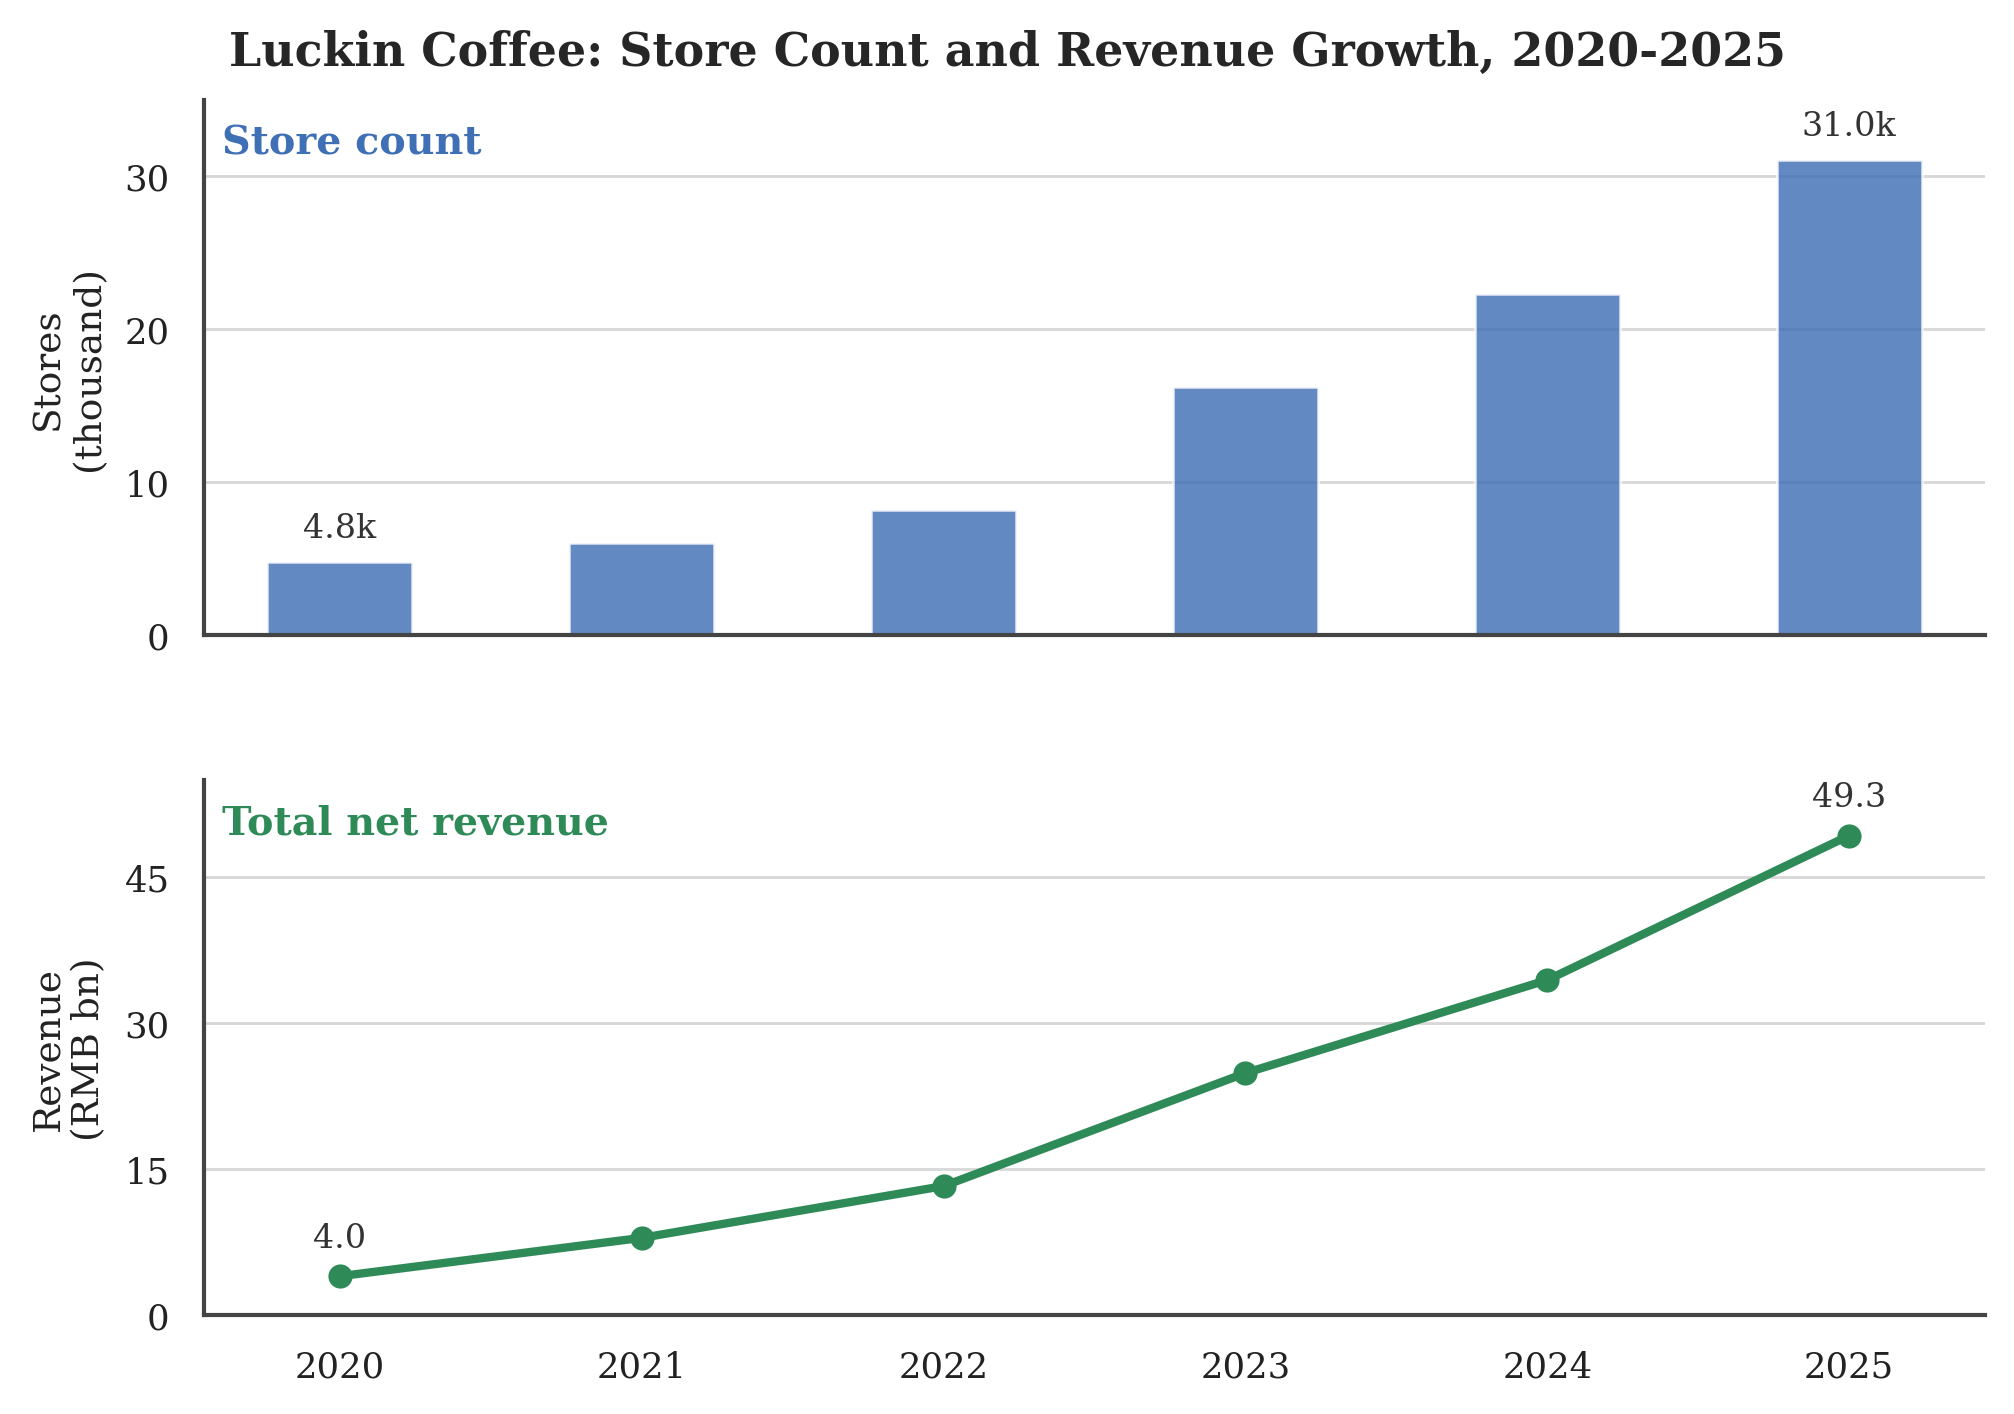
\includegraphics[width=0.9\textwidth]{fig_growth.png}
  \caption{Luckin Coffee store count and revenue growth (2020--2025).\label{fig:growth}}
\end{figure}

% =================== III. BUSINESS ANALYSIS ===================
\section{Business Analysis}

The following analysis adopts a multi-perspective framework grounded in the management domains pertinent to enterprise architecture. Drawing on strategic management as an organising lens, this section examines the enterprise through five interrelated dimensions: stakeholders, customers, financial architecture, internal business processes, and organisational learning and growth.

\subsection{Stakeholders and Key Partners}

Luckin's stakeholder ecosystem is both expansive and densely interconnected, reflecting the operational complexity inherent in managing a network of over thirty thousand physical points of sale integrated with a unified digital infrastructure. The principal stakeholder categories include:

\begin{figure}[H]
  \centering
  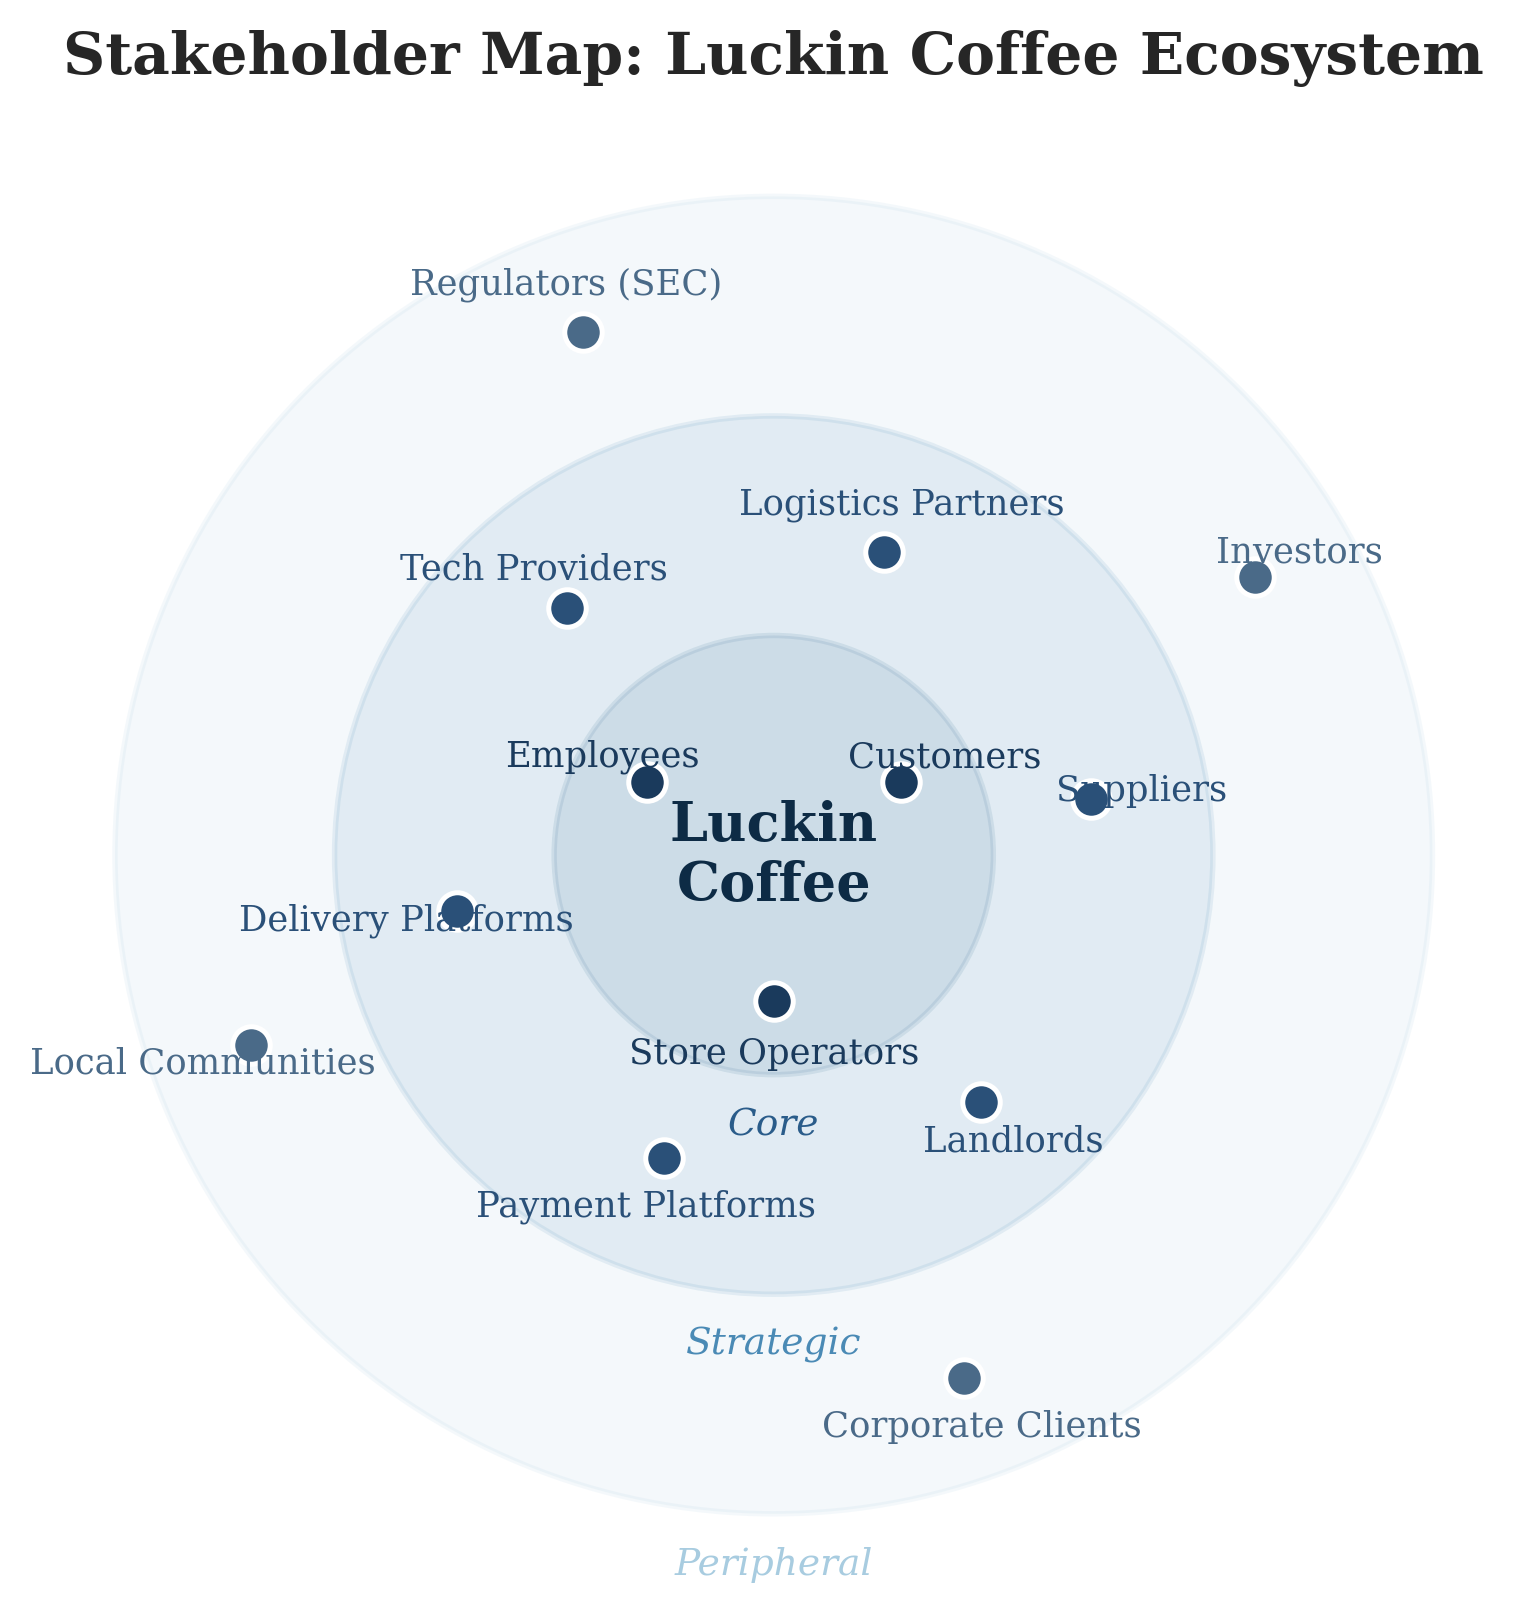
\includegraphics[width=0.85\textwidth]{fig_stakeholders.png}
  \caption{Stakeholder map of Luckin Coffee's ecosystem.\label{fig:stakeholders}}
\end{figure}

\begin{itemize}[leftmargin=*]
  \item \textbf{Upstream supply chain partners:} coffee bean producers and exporters spanning multiple origins (Brazil, Colombia, Ethiopia, Honduras, Tanzania, and Yunnan, China), raw material suppliers, packaging manufacturers, and third-party logistics providers responsible for warehousing and fulfilment.
  \item \textbf{Operational partners:} partnership-store operators (franchisees) who extend the brand's geographic reach while bearing a proportion of capital expenditure; delivery platform providers (both proprietary and third-party) that execute last-mile fulfilment.
  \item \textbf{Technology and platform partners:} payment processing platforms (WeChat Pay, Alipay), cloud infrastructure providers, and software service vendors that support application development and data analytics capabilities.
  \item \textbf{Downstream and institutional stakeholders:} end consumers, corporate clients, landlords and property lessors, equity investors and debt holders, financial regulators (including the U.S.\ Securities and Exchange Commission, given the company's continued reporting obligations under Form~20-F), and the local communities in which stores operate.
\end{itemize}

From an enterprise architecture perspective, the integration of supply chain management systems, warehouse management systems, order management platforms, and store-level operational data constitutes a critical architectural concern. Luckin's investments in proprietary roasting facilities in Fujian, Jiangsu, and Yunnan further indicate that vertical integration of the upstream value chain is a deliberate strategic priority, with direct implications for system interoperability and data governance.

\subsection{Customers: Typology, Relationship Architecture, and Channels}

Luckin addresses the mass-market coffee and beverage segment. Its customer base can be classified into the following categories:

\begin{enumerate}[leftmargin=*,label=(\roman*)]
  \item \textbf{Office workers} who prioritise speed and convenience, typically ordering via mobile application for rapid pickup during commute windows or lunch breaks.
  \item \textbf{University students and young consumers} drawn by accessible price points, promotional campaigns, and social-media-driven brand engagement.
  \item \textbf{Commuters and on-the-go consumers} who utilise delivery or pickup services based on situational convenience.
  \item \textbf{Corporate and institutional clients} that procure beverages for employees through Luckin's enterprise account functionality.
\end{enumerate}

The customer relationship model is fundamentally digital and data-intensive. Consumer touchpoints are concentrated within the proprietary mobile application, the WeChat mini-program ecosystem, and, to a secondary extent, third-party delivery aggregators. The application architecture supports a comprehensive suite of functionalities: location-based store recommendation, menu customisation, digital payment processing, pickup-versus-delivery selection, real-time order tracking, and post-transaction feedback collection. This digital-native interface architecture gives Luckin a direct relationship with its customers, enabling the firm to leverage order histories, consumption preferences, personalised voucher distribution, and behavioural segmentation to drive repeat purchase frequency and customer lifetime value.

\subsection{Financial Architecture}

Luckin's revenue architecture reflects its hybrid operating model, wherein two distinct revenue streams coexist:

\begin{figure}[H]
  \centering
  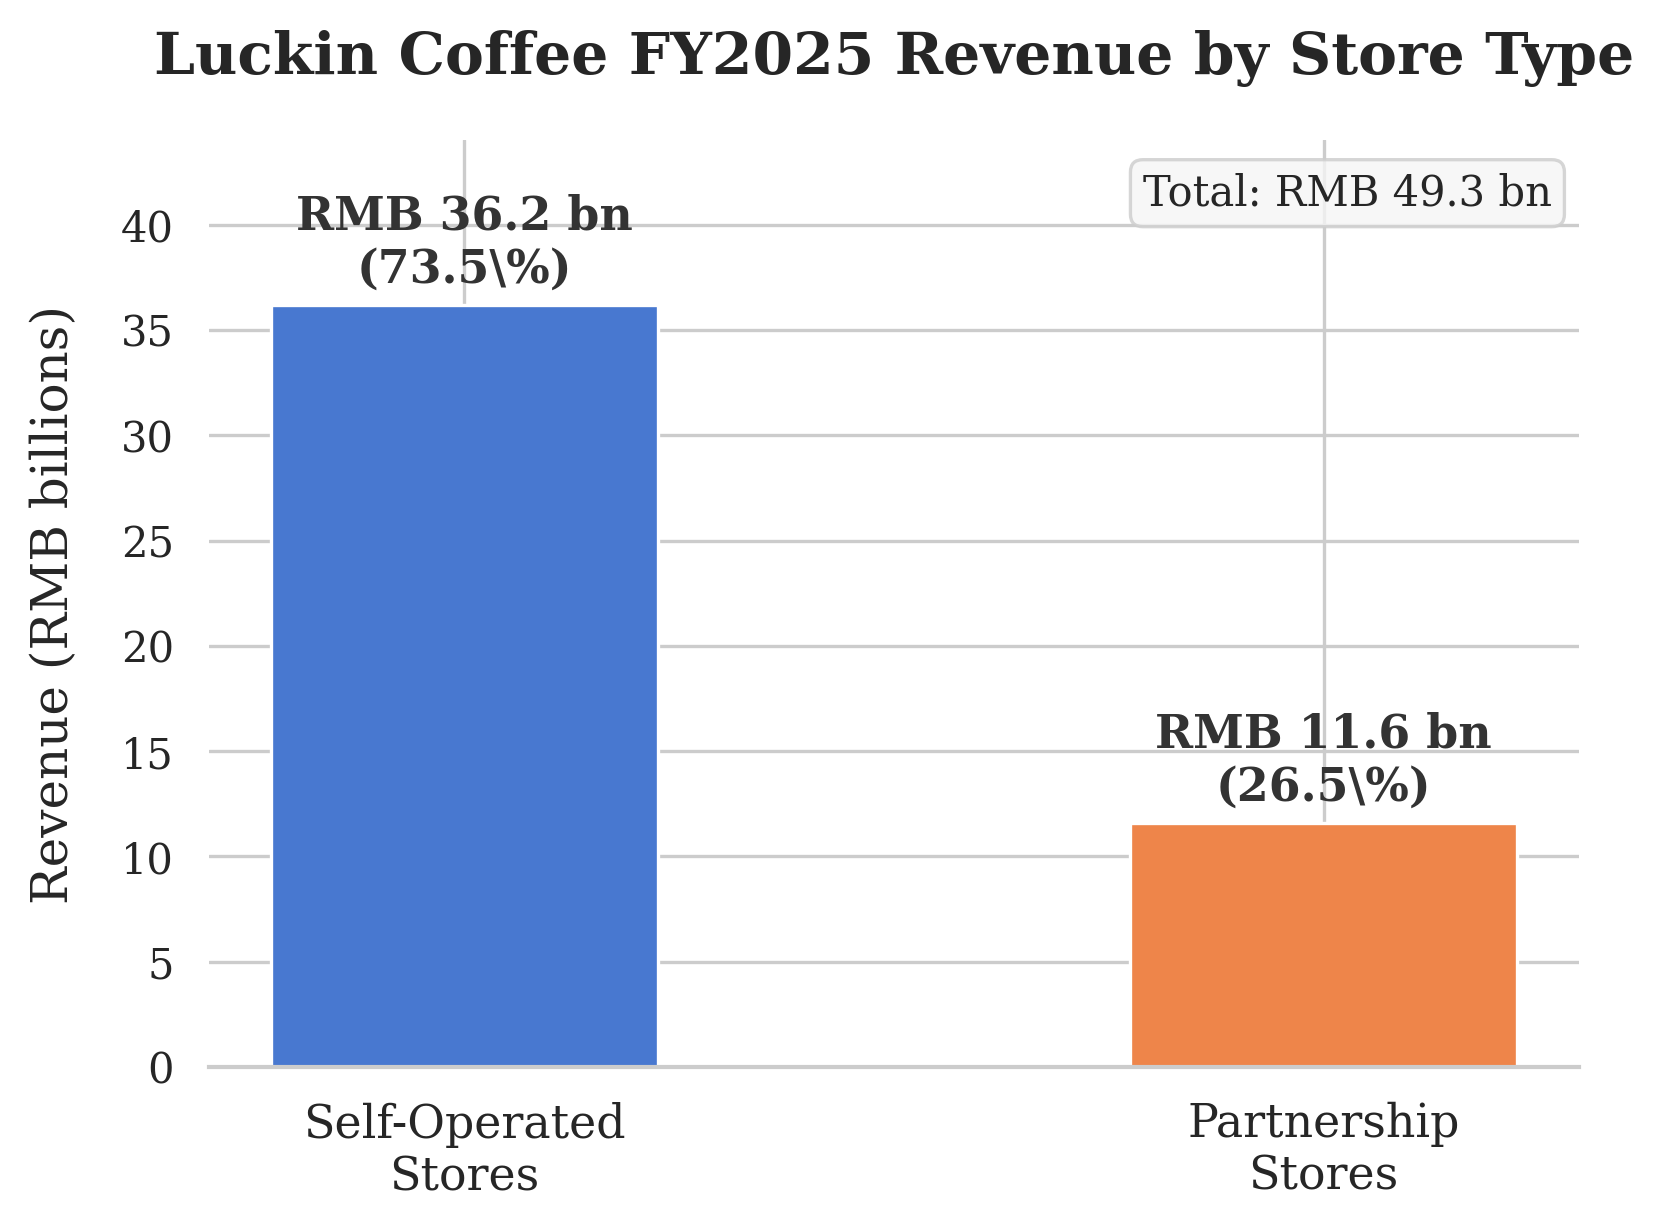
\includegraphics[width=0.65\textwidth]{fig_revenue.png}
  \caption{Luckin Coffee FY2025 revenue by store type. Source: Luckin Coffee 2025 Form~20-F.\label{fig:revenue}}
\end{figure}

\begin{enumerate}[leftmargin=*,label=(\arabic*)]
  \item \textbf{Self-operated store revenue} (RMB~36.2 billion in FY2025, representing approximately 73.5\% of total net revenue): generated through direct product sales of freshly brewed beverages, other food and beverage items, delivery service charges, e-commerce sales of packaged coffee products, and ancillary income.
  \item \textbf{Partnership store revenue} (RMB~11.6 billion in FY2025): derived from sales of raw materials and equipment to franchise operators, delivery service fees, profit-sharing arrangements, royalty payments, initial franchise fees, and other service-related charges.
\end{enumerate}

This dual-structure model offers strategic advantages: self-operated stores give the firm direct control over brand standards, service quality, and data capture, while partnership stores facilitate accelerated geographic expansion with attenuated capital intensity. The cost structure is correspondingly multifaceted, with principal cost categories encompassing raw material procurement, store-level rent and occupancy costs, direct and indirect labour, utilities, depreciation of property and equipment, delivery and fulfilment expenses, sales and marketing expenditure, general and administrative overhead, and ongoing research and development investment.

For FY2025, Luckin reported GAAP operating income of RMB~5.1 billion, corresponding to an operating margin of 10.3\%. This metric signals a transition from a growth-at-all-costs posture toward a more mature, profitability-oriented operating model. From an enterprise architecture standpoint, the financial dimension interfaces with data systems through revenue recognition, cost allocation, inventory valuation, and store-level profitability analytics---all of which depend on the integrity and integration of transactional and operational data flows.

\subsection{Internal Business Processes}

Luckin's internal process architecture can be delineated as an end-to-end value chain encompassing the following core functions:

\begin{figure}[H]
  \centering
  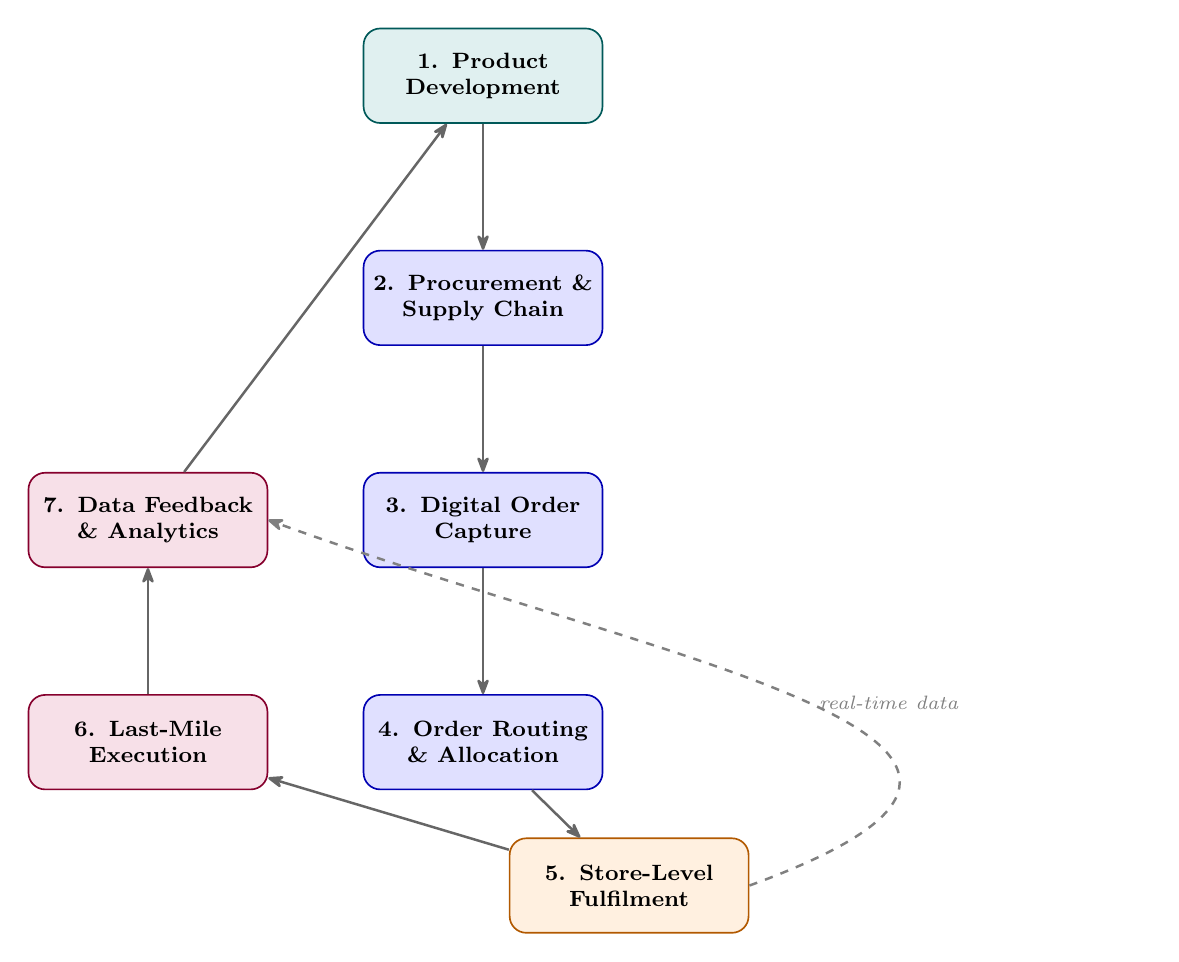
\begin{tikzpicture}[
    node distance=1.6cm and 1.2cm,
    box/.style={rectangle, rounded corners=6pt, draw=#1!70!black, fill=#1!12,
                text width=2.8cm, align=center, minimum height=1.2cm,
                font=\footnotesize\bfseries, line width=0.6pt},
    arrow/.style={-{Stealth[round]}, line width=0.9pt, black!60},
  ]
  % --- Top: Product Dev ---
  \node[box=teal] (dev) {1. Product\\Development};

  % --- Right column ---
  \node[box=blue, below=of dev] (proc) {2. Procurement \&\\Supply Chain};
  \node[box=blue, below=of proc] (order) {3. Digital Order\\Capture};
  \node[box=blue, below=of order] (route) {4. Order Routing\\\& Allocation};

  % --- Bottom ---
  \node[box=orange, below right=0.6cm and -1.2cm of route] (store) {5. Store-Level\\Fulfilment};

  % --- Left column ---
  \node[box=purple, left=of route] (last) {6. Last-Mile\\Execution};
  \node[box=purple, above=of last] (data) {7. Data Feedback\\\& Analytics};

  % --- Arrows ---
  \draw[arrow] (dev) -- (proc);
  \draw[arrow] (proc) -- (order);
  \draw[arrow] (order) -- (route);
  \draw[arrow] (route) -- (store);
  \draw[arrow] (store) -- (last);
  \draw[arrow] (last) -- (data);
  \draw[arrow] (data) -- (dev);

  % --- Dashed feedback loop annotation ---
  \draw[arrow, dashed, gray] (store.east) to[out=20, in=-20, looseness=1.8]
    node[midway, right, font=\scriptsize\itshape, text=gray]{real-time data} (data.east);

  \end{tikzpicture}
  \caption{End-to-end business process architecture of Luckin Coffee. Each stage is mediated by dedicated information systems, forming a closed-loop data-driven operating model.\label{fig:process}}
\end{figure}

As illustrated in Figure~\ref{fig:process}, each stage of Luckin's value chain is mediated by information systems: product lifecycle management tools, procurement and warehouse management platforms, order management systems, in-store point-of-sale and production terminals, delivery coordination software, and customer analytics engines. The dashed feedback loop---whereby post-transaction data on customer ratings, delivery performance, and consumption patterns are continuously routed back into product development, demand forecasting, and marketing campaign design---is a defining architectural feature. This tight coupling of physical operations with digital information flows renders Luckin an instructive case study in business--IT alignment.

\subsection{Learning and Growth}

The learning and growth dimension captures the organisation's capacity for continuous improvement, innovation, and adaptive change. Luckin's capabilities in this domain are manifested across four interrelated areas:

\begin{enumerate}[leftmargin=*,label=(\alph*)]
  \item \textbf{Product Innovation Velocity:} The firm maintains an aggressive new product introduction cadence, launching numerous stock-keeping units (SKUs) annually. Flagship products serve as both revenue drivers and brand-building vehicles, and the innovation pipeline is informed by real-time sales data and consumer preference analytics.
  \item \textbf{Digital Feedback Infrastructure:} The digital ordering model generates rapid, granular feedback loops. Sales velocity data reveals product-market fit; customer segmentation enables precision marketing; delivery and pickup analytics inform site-selection and store-density optimisation; and store-level performance dashboards support expansion and operational decisions. This data infrastructure is a key driver of organisational learning.
  \item \textbf{Standardised Training and Human Capital Development:} Standardised operational procedures, supported by digital training modules and in-store coaching, enable the rapid onboarding of store personnel and facilitate consistent execution across a geographically dispersed store network.
  \item \textbf{Technology Investment and System Evolution:} Luckin sustains ongoing investment in its application ecosystem, warehouse management capabilities, supply chain digitisation, and operational support systems, demonstrating that the company views technology as a key competitive advantage.
\end{enumerate}

Notwithstanding these capabilities, the firm confronts several challenges relevant to the learning and growth perspective: intense price competition within the Chinese beverage market, structural cost pressures associated with delivery-dependent orders, the operational complexity of quality assurance across a store network exceeding thirty thousand locations, the managerial demands of international market entry, and the enduring reputational legacy of the 2020 accounting irregularities. These challenges represent significant variables in any assessment of the firm's adaptive capacity and long-term resilience.

% =================== CLOSING REMARK ===================
\vspace{0.5cm}
\noindent
The foregoing analysis establishes Luckin Coffee as a compelling subject for enterprise architecture investigation. The firm's competitive posture rests not on any single operational capability, but on the systemic alignment of business strategy, digital channel architecture, supply chain integration, store operations, and data-driven management processes. This dense web of interdependencies between strategic intent and technological execution provides fertile ground for subsequent architectural modelling and database design inquiry.

\end{document}
